\documentclass[a4paper,12pt]{report}
\usepackage[T2A]{fontenc}
\usepackage[utf8]{inputenc}
\usepackage[english,russian]{babel}
\usepackage{graphicx}
\usepackage{wrapfig}
\usepackage{mathtext} 				% русские буквы в фомулах
\usepackage{amsmath,amsfonts,amssymb,amsthm,mathtools} % AMS
\usepackage{icomma} % "Умная" запятая: $0,2$ --- число, $0, 2$ --- перечисление
\usepackage{capt-of}
\usepackage{appendix}
\usepackage{multirow}
\usepackage{hyperref}
\usepackage{floatrow}
\usepackage[left=2cm,right=2cm,
    top=2cm,bottom=2cm,bindingoffset=0cm]{geometry}
\usepackage{multicol} % Несколько колонок
\usepackage{gensymb}
\title{Отчёт по лабораторной работе № 5.1.3. 

Изучение рассеяния медленных электронов на атомах (эффект Рамзауэра).}
\author{Плюскова Н.А. Б04-004 }
\date{\today}
\begin{document}
\maketitle
\section*{1. Аннотация}
В данной работе была исследована энергетическая зависимость вероятности рассеяния электронов атомами ксенона, при которых наблюдается "просветление" ксенона, а также был оценен размер его внешней электронной оболочки


\section*{2. Теоретические сведения}
К. Рамзауэр исследовал зависимость поперечных сечений упрогого рассеяния электронов (с энергией до 10 ЭВ) на атомах аргона. В результате этих исследований было обнаружено явление, получившее название \textit{эффекта Рамзауэра}.
	
	С точки зрения квантовой теории атом по отношению к электронной волне ведет себя как преломляющая среда с относительным показателем преломления
	\begin{equation*}
		n = \frac{\lambda}{\lambda^\prime} = \sqrt{1-\frac{U}{E}},
	\end{equation*}
	где $U$, $E$ -- соответственно потенциальная и полная энергии электрона внутри атома.
	
	Будем считать, что электрон рассеивается на одномерной прямоугольной потенциальной яме конечной глубины. Такая модель является хорошим приближением для атомов тяжелых инертных газов, отличающихся наиболее компактной структурой и резкой внешней границей.
	
	Коэффициент прохождения равен отношению квадратов амплитуд прошедшей и падающей волн и определяется выражением:
	\begin{equation*}
		\frac{1}{D} = 1 + \frac{U_0^2}{4E(E+U_0)}\sin^2(k_2l).
	\end{equation*}
	Минимум последнего выражения отвечает квантовому аналогу просветления оптики, так как при выполнении условия
	\begin{equation*}
		\tag{$\star$}
		\label{eq:uslovie}
		\sqrt{\frac{2m(E+U_0)}{\hbar^2}}l = \pi n, \ n\in\mathbb{N},
	\end{equation*}
	коэффициент прохождения частицы над ямой становится равным единице, то есть достигает своего максимального значения.
	Отметим, что условие~(\ref{eq:uslovie}) легко получить, рассматривая интерференцию электронов волн де Бройля в атоме:\\
	\begin{itemize}
		\item
			Условие первого интерференционного максимума:
			\begin{equation}
				\label{eq:1}
				2l = \frac{h}{\sqrt{2m(E_1+U_0)}}.
			\end{equation}
		\item
			Условие первого интерференционного минимума:
			\begin{equation}
				\label{eq:2}
				2l =\frac{3}{2} \frac{h}{\sqrt{2m(E_2+U_0)}}.
			\end{equation}			
	\end{itemize}

	Решая совместно уравнения~(\ref{eq:1}, \ref{eq:2}) можно получить:
	\begin{equation}
		\label{eq:l}
		l = \frac{h\sqrt{5}}{\sqrt{32m(E_2-E_1)}}.
	\end{equation}
	Здесь энергии $E_1$ и $E_2$ соответствуют энергиям электронов, прошедших разность потенциалов $V_1$ и $V_2$, то есть $E_1 = eV_1$ и $E_2 = eV_2$. 
	
	По измеренным величинам $E_1$ и $E_2$, используя формулы~(\ref{eq:1}, \ref{eq:2}), можно рассчитать эффективную глубину потенциальной ямы атома:
	\begin{equation}
		\label{eq:U_0}
		U_0 = \frac{4}{5}E_2 - \frac{9}{5}E_1
	\end{equation}

	Согласно квантовой механике зависимость вероятности рассеяния электрона от его энергии можно определить из соотношения:
	\begin{equation}
		\label{eq:w}
		w(U) = -\frac{1}{C}\ln \frac{I(U)}{I_0},
	\end{equation}
	где $I_0$ -- ток катода, а $C$ -- некторая постоянная.

\section*{3. Экспериментальная установка}

	В нашей работе для изучения эффекта Рамзауэра используется тиратрон ТГ3-01/1.3Б, заполненный инертным газом. Схематическое изображение тиратрона и его конструкция приведены на рис.1.
	
	Принципиальная схема установки для изучения эффекта Рамзауэра приведена на рис.2. На лампу Л подаётся синусоидальное напряжение частоты 50 Гц от источника питания ИП, С -- стабилизированный блок накала катода; исследуемый сигнал подаётся на электронный осциллограф (ЭО); цифрами обозначены номера ножек лампы.
	
	\begin{figure}[H]
    \centering
    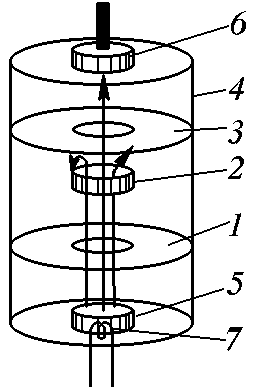
\includegraphics[width=4 cm]{pic1.png}
    \caption{Устройство тиратрона}
    \label{fig:vac}
\end{figure}

\begin{figure}[H]
    \centering
    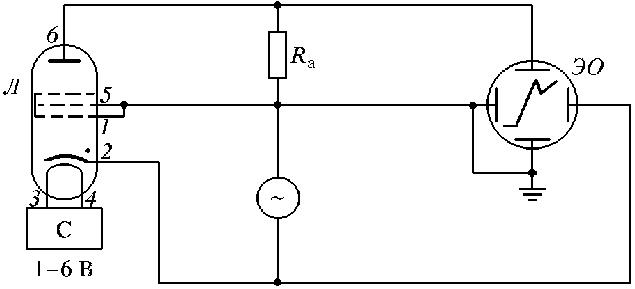
\includegraphics[width=8cm]{pic2.png}
    \caption{Экспериментальная установка
    }
    \label{fig:vac}
\end{figure}

	
	Схема экспериментальной установки, изображённая на рис.2 в нашей работе конструктивно осуществлена следующим образом. Лампа-тиратрон ТГ3-01/1.3Б, заполненная инертным газом, расположена непосредственно на корпусе блока источника питания (БИП). Напряжение к электродам лампы подаётся от источников питания, находящихся в корпусе прибора. Регулировка напряжения и выбор режима работы установки производится при помощи ручек управления, выведенных на лицевую панель БИП.
	
\section*{4. Ход работы}
\subsection*{4.1 Измерение ВАХ тиратрона на экране осциллографа}
Измерим на экране осциллографа напряжения между катодом и сеткой, соответствующие первому максимуму и минимуму на осциллограмме, а также оценим напряжение пробоя, соответствующее резкому скачку тока в конце кривой (рис.3 и рис.4):

\begin{table}[H]
\begin{tabular}{|c|c|c|c|c|c|c|c|}
\hline
$U_{\text{накал}}$, В & $\sigma_{U_{\text{накал}}}$, В              & $V_max$,В & $\sigma_{V_{max}}$,В          & $V_min$,В & $\sigma_{V_{min}}$,В & $V_{\text{пробоя}}$, В & $\sigma_{V_{\text{пробоя}}}$, В \\ \hline
2,520     & \multirow{2}{*}{0,003} & 1,6    & \multirow{2}{*}{0,2} & 8,0    & 0,8         & 14,0       & 1,0             \\ \cline{1-1} \cline{3-3} \cline{5-8} 
2,849     &                        & 2,0    &                      & 7,4    & 0,4         & 12,4       & 1,1             \\ \hline
\end{tabular}
\caption{Измерение ВАХ тиратрона на экране осциллографа}
\end{table}

Рассчитаем размер электронной оболочки атома инертного газа, заполняющего лампу, приняв $U_{0} = 2,5$ В по формулам (1) и (2):

\begin{table}[H]
\begin{tabular}{|c|c|c|}
\hline
$U_{\text{накала}}$, В & $l, \textup{~\AA}$ & $\sigma_{l}, \textup{~\AA}$ \\ \hline
2,52       & 2,84 & 0,15      \\ \hline
2,85       & 2,98 & 0,21      \\ \hline
\end{tabular}
\end{table}

Рассчитаем размер электронной оболочки атома по формуле (3):

\begin{table}[H]
\begin{tabular}{|c|c|c|}
\hline
$U_{\text{накала}}$, В & $l, \textup{~\AA}$ & $\sigma_{l}, \textup{~\AA}$\\ \hline
2,52       & 2,46 & 0,17      \\ \hline
2,85       & 2,56 & 0,12      \\ \hline
\end{tabular}
\caption{Расчет электронной оболочки атома для двух значений $U_{\text{накала}}$}
\end{table}

Тогда $l \approx (2,51 \pm 0,17) \textup{~\AA}$, что в пределах $2\sigma$ (теоретическое значение 2,8$\textup{~\AA}$)

Заметим, что размер электронной оболочки атома, рассчитанный первым способом, больше, чем вторым. Это связано с тем, что глубина потенциальной ямы $U_0$ на самом деле отличается от 2,5 В.

Оценим глубину потенциальной ямы по формуле (4):

\begin{table}[H]
\begin{tabular}{|c|c|c|}
\hline
$U_{\text{накала}}$, В  & $U_0$, В & $\sigma_{U_0}$, В \\ \hline
2,52       & 3,52  & 0,87       \\ \hline
2,85       & 2,16  & 0,63       \\ \hline
\end{tabular}
\end{table}

Получим, что $U_0 \approx (2,84\pm 0,87)$ В, т.е. глубина потенциальной ямы на самом деле больше, чем 2,5 В.

Как видно из таблицы 1 $V_{\text{пробоя}}\approx (13,2 \pm 1,1)$ В, что похоже на ионизационный потенциал ксенона.

\begin{figure}[H]
    \centering
    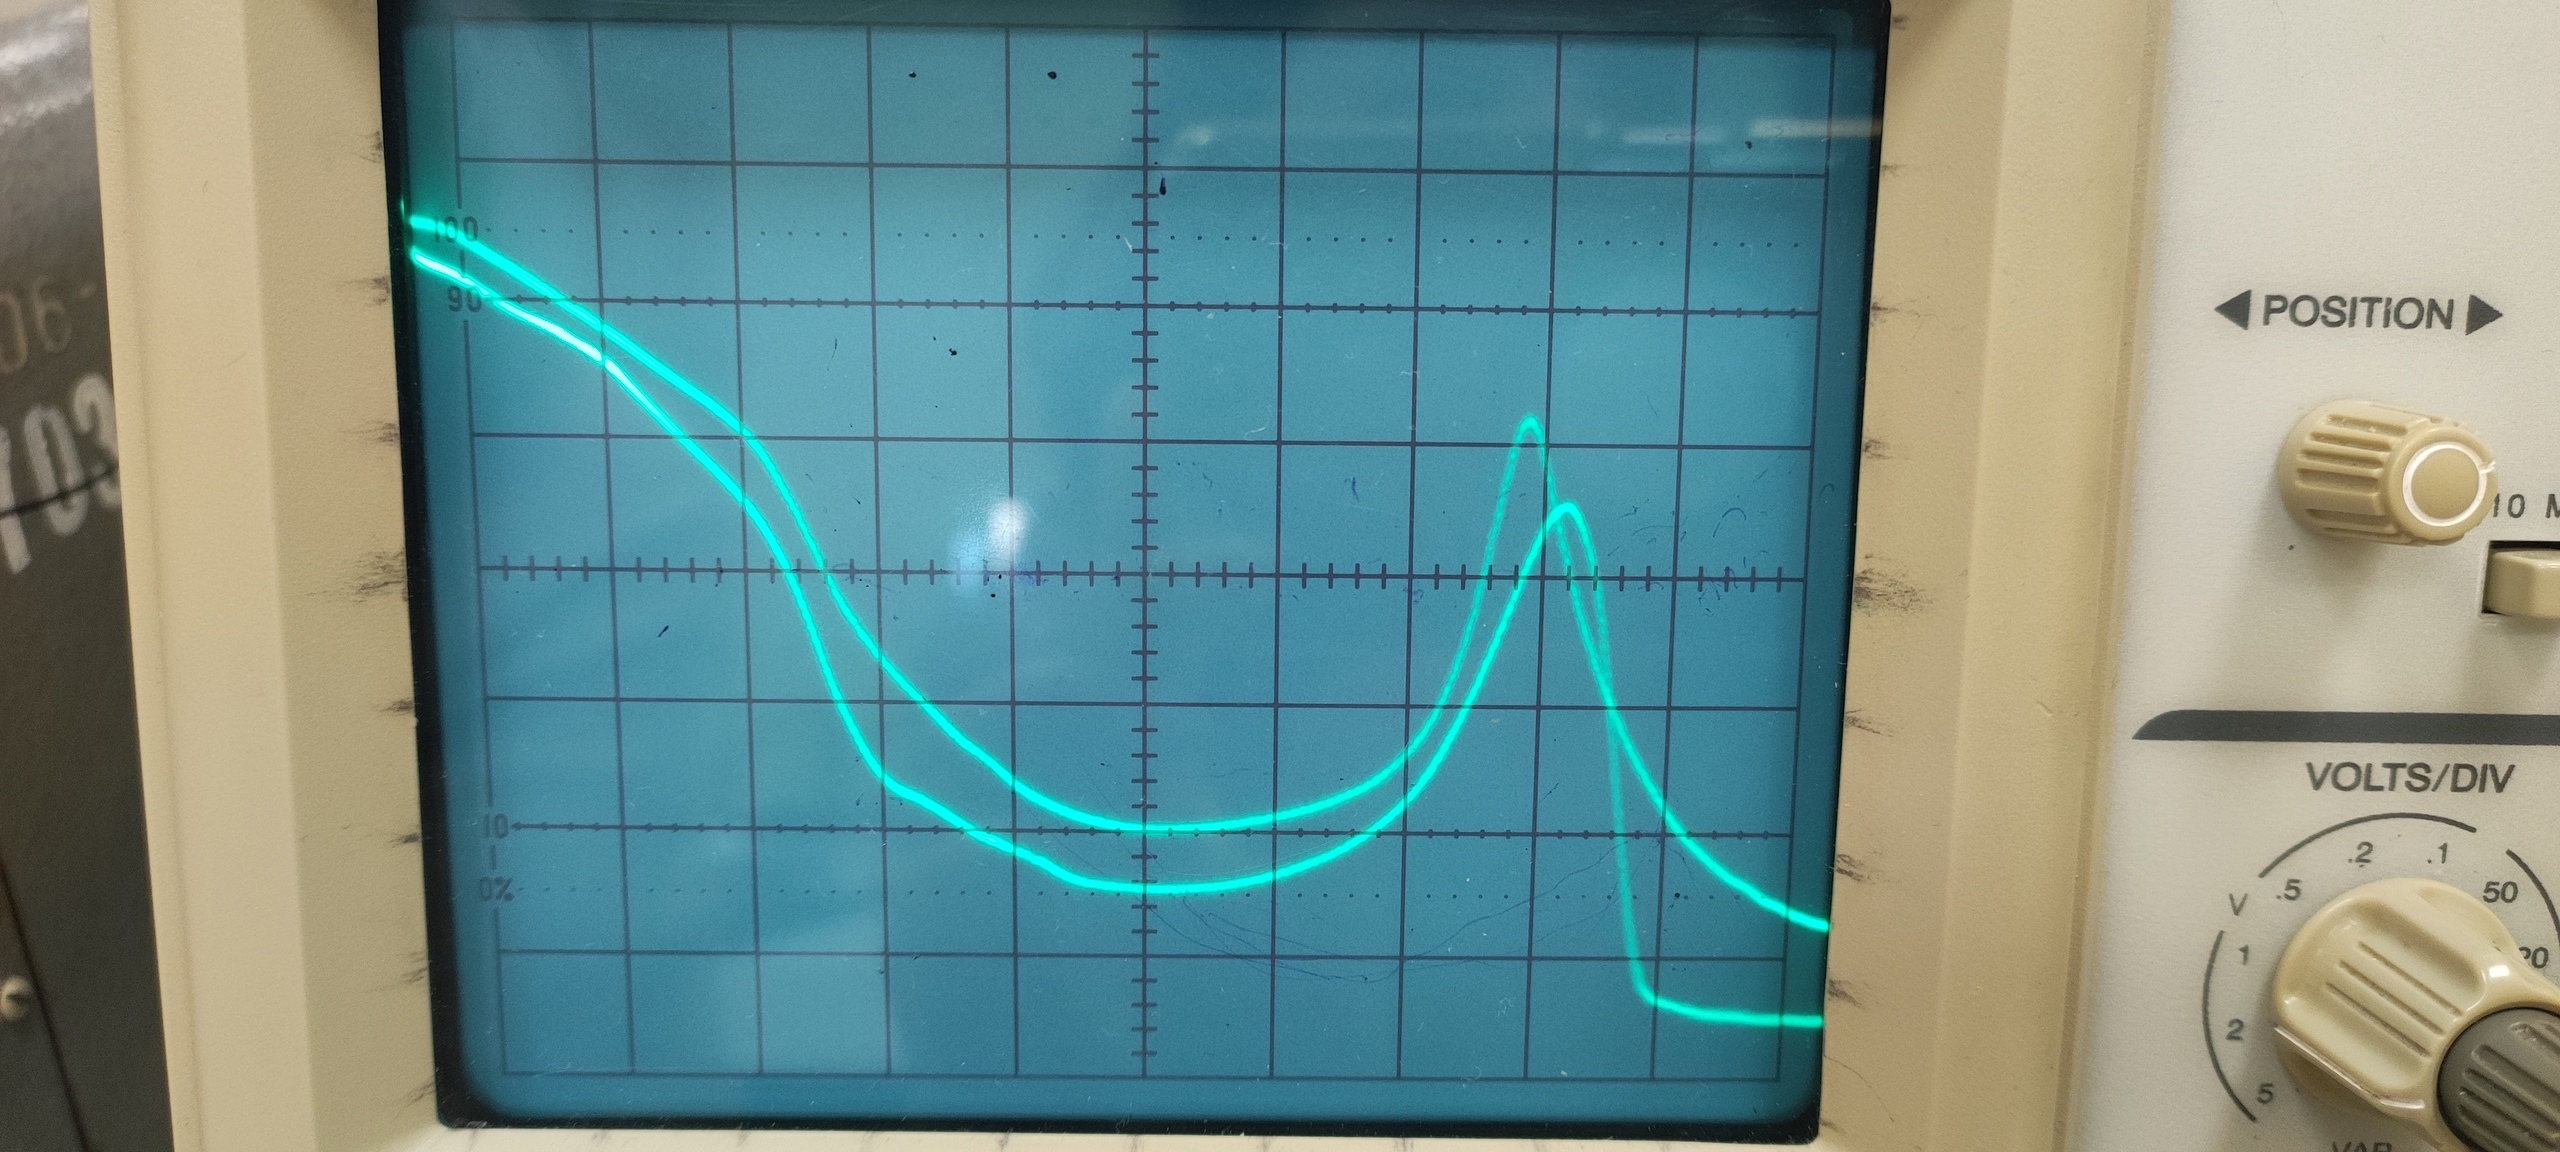
\includegraphics[width=14cm]{pic1.jpg}
    \caption{Измерение ВАХ на экране осциллографа}
    \label{fig:vac}
\end{figure}
\begin{figure}[H]
    \centering
    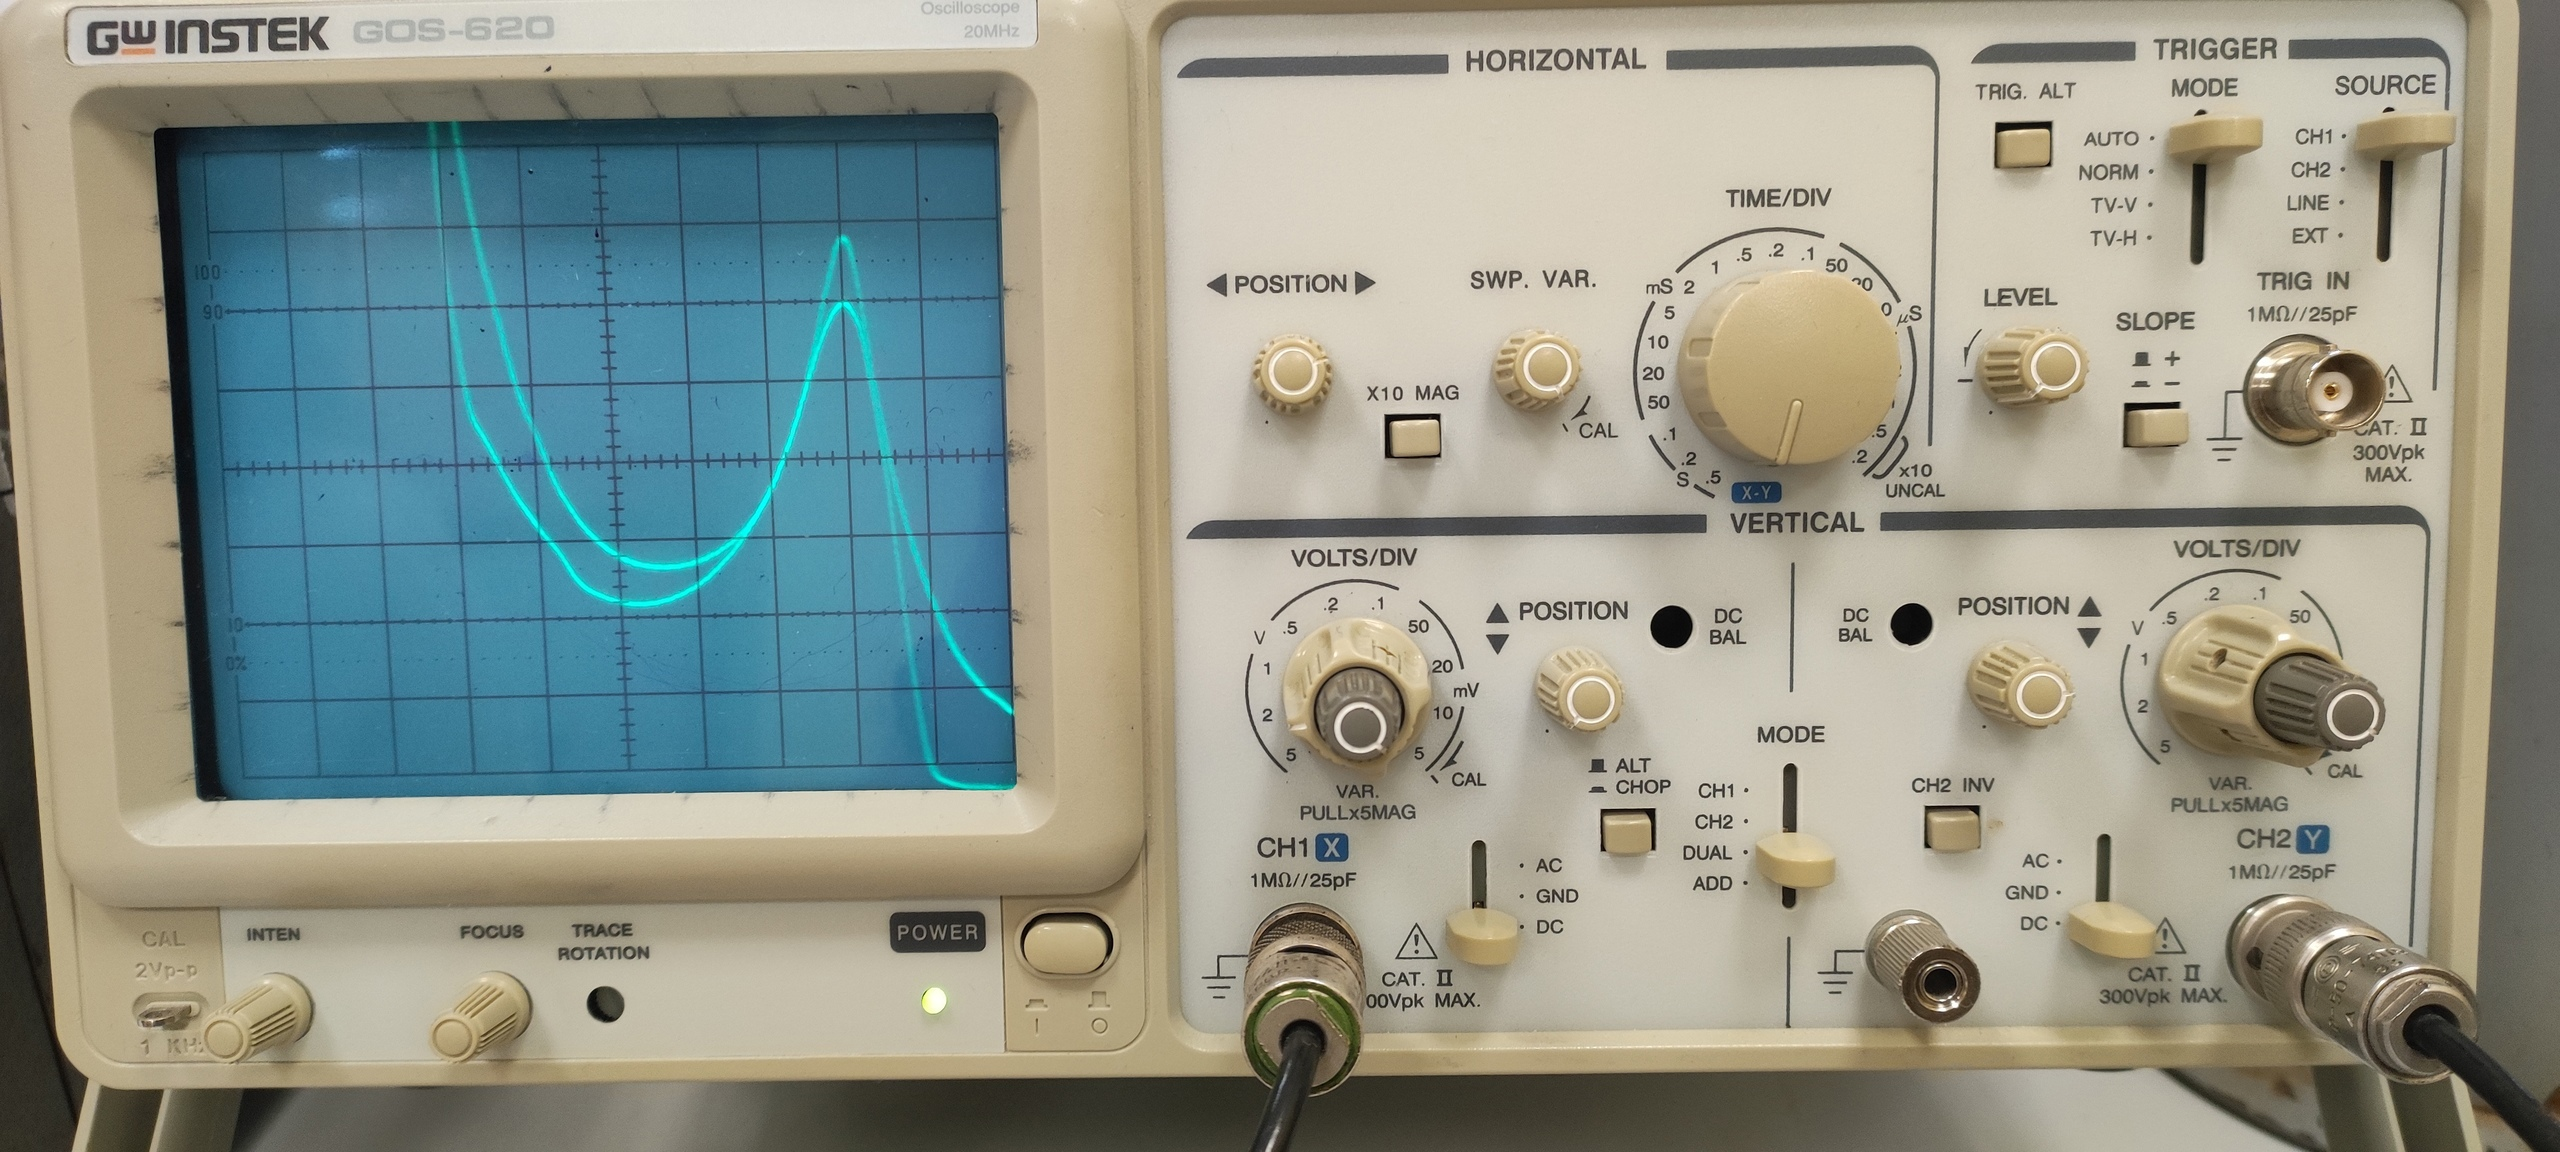
\includegraphics[width=14cm]{pic2.jpg}
    \caption{Измерение ВАХ на экране осциллографа}
    \label{fig:vac}
\end{figure}

\subsection*{4.2 Измерение ВАХ в статическом режиме}
Проведем измерение ВАХ тиратрона для 2-х значений напряжения накала.

\begin{table}[H]
\begin{tabular}{|c|c|c|c|}
\hline
$V$,В  & $\sigma_V$, В              & $I_a, \cdot 10^{-3}$ мкА  & $\sigma_{I_{a}},\cdot10^{-3}$ мкА           \\ \hline
0,20 & \multirow{21}{*}{0,01} & -0,1   & \multirow{21}{*}{0,1} \\ \cline{1-1} \cline{3-3}
0,30 &                        & -0,6   &                       \\ \cline{1-1} \cline{3-3}
0,43 &                        & -0,3   &                       \\ \cline{1-1} \cline{3-3}
0,53 &                        & 0,9    &                       \\ \cline{1-1} \cline{3-3}
0,69 &                        & 8,0    &                       \\ \cline{1-1} \cline{3-3}
0,58 &                        & 2,0    &                       \\ \cline{1-1} \cline{3-3}
0,65 &                        & 5,2    &                       \\ \cline{1-1} \cline{3-3}
0,72 &                        & 12,1   &                       \\ \cline{1-1} \cline{3-3}
0,78 &                        & 23,1   &                       \\ \cline{1-1} \cline{3-3}
0,81 &                        & 31,0   &                       \\ \cline{1-1} \cline{3-3}
0,87 &                        & 55,9   &                       \\ \cline{1-1} \cline{3-3}
0,89 &                        & 67,6   &                       \\ \cline{1-1} \cline{3-3}
0,91 &                        & 79,7   &                       \\ \cline{1-1} \cline{3-3}
0,92 &                        & 88,5   &                       \\ \cline{1-1} \cline{3-3}
0,94 &                        & 104,5  &                       \\ \cline{1-1} \cline{3-3}
1,10 &                        & 315,2  &                       \\ \cline{1-1} \cline{3-3}
1,21 &                        & 521,9  &                       \\ \cline{1-1} \cline{3-3}
1,43 &                        & 1039,9 &                       \\ \cline{1-1} \cline{3-3}
1,63 &                        & 1419,8 &                       \\ \cline{1-1} \cline{3-3}
1,87 &                        & 1472,8 &                       \\ \cline{1-1} \cline{3-3}
2,08 &                        & 1267,2 &                       \\ \hline

2,24  & \multirow{12}{*}{0,01} & 1102,6 & \multirow{21}{*}{0,1} \\ \cline{1-1} \cline{3-3}
2,45  &                        & 910,7  &                       \\ \cline{1-1} \cline{3-3}
2,67  &                        & 756,4  &                       \\ \cline{1-1} \cline{3-3}
2,83  &                        & 664,0  &                       \\ \cline{1-1} \cline{3-3}
3,04  &                        & 576,4  &                       \\ \cline{1-1} \cline{3-3}
3,27  &                        & 505,6  &                       \\ \cline{1-1} \cline{3-3}
3,63  &                        & 417,2  &                       \\ \cline{1-1} \cline{3-3}
4,16  &                        & 334,9  &                       \\ \cline{1-1} \cline{3-3}
4,51  &                        & 302,9  &                       \\ \cline{1-1} \cline{3-3}
4,95  &                        & 271,1  &                       \\ \cline{1-1} \cline{3-3}
5,60  &                        & 242,6  &                       \\ \cline{1-1} \cline{3-3}
6,08  &                        & 232,0  &                       \\ \cline{1-3}
6,40  & \multirow{2}{*}{0,1}   & 237,0  &                       \\ \cline{1-1} \cline{3-3}
7,00  &                        & 232,0  &                       \\ \cline{1-3}
7,82  & \multirow{7}{*}{0,01}  & 240,1  &                       \\ \cline{1-1} \cline{3-3}
8,40  &                        & 254,0  &                       \\ \cline{1-1} \cline{3-3}
8,99  &                        & 275,1  &                       \\ \cline{1-1} \cline{3-3}
9,67  &                        & 332,0  &                       \\ \cline{1-1} \cline{3-3}
10,21 &                        & 395,3  &                       \\ \cline{1-1} \cline{3-3}
11,07 &                        & 456,0  &                       \\ \cline{1-1} \cline{3-3}
11,60 &                        & 535,0  &                       \\ \hline
\end{tabular}
\caption{Измерение ВАХ в статическом режиме при $U_{\text{накала}}=$ 2,52 В}
\end{table}

\begin{table}[H]
\begin{tabular}{|c|c|c|c|}
\hline
$V$,В  & $\sigma_V$, В              & $I_a, \cdot 10^{-3}$ мкА  & $\sigma_{I_{a}},\cdot10^{-3}$ мкА    \\ \hline
0,43 & \multirow{14}{*}{0,01} & 1,5             & \multirow{14}{*}{0,1}  \\ \cline{1-1} \cline{3-3}
0,85 &                        & 127,6           &                        \\ \cline{1-1} \cline{3-3}
0,99 &                        & 314             &                        \\ \cline{1-1} \cline{3-3}
1,10 &                        & 530,9           &                        \\ \cline{1-1} \cline{3-3}
1,18 &                        & 727,7           &                        \\ \cline{1-1} \cline{3-3}
1,26 &                        & 962,8           &                        \\ \cline{1-1} \cline{3-3}
1,45 &                        & 1410,5          &                        \\ \cline{1-1} \cline{3-3}
1,66 &                        & 1731,4          &                        \\ \cline{1-1} \cline{3-3}
1,82 &                        & 1779,5          &                        \\ \cline{1-1} \cline{3-3}
2,06 &                        & 1665,9          &                        \\ \cline{1-1} \cline{3-3}
2,31 &                        & 1482,7          &                        \\ \cline{1-1} \cline{3-3}
2,55 &                        & 1337,3          &                        \\ \cline{1-1} \cline{3-3}
2,73 &                        & 1249,3          &                        \\ \cline{1-1} \cline{3-3}
3,25 &                        & 1056,4          &                        \\ \hline

3,61  & \multirow{14}{*}{0,01} & 962,1           & \multirow{14}{*}{0,1}  \\ \cline{1-1} \cline{3-3}
3,89  &                        & 934,1           &                        \\ \cline{1-1} \cline{3-3}
4,40  &                        & 831,6           &                        \\ \cline{1-1} \cline{3-3}
5,04  &                        & 772,6           &                        \\ \cline{1-1} \cline{3-3}
5,60  &                        & 745,3           &                        \\ \cline{1-1} \cline{3-3}
6,11  &                        & 735,1           &                        \\ \cline{1-1} \cline{3-3}
6,75  &                        & 742,1           &                        \\ \cline{1-1} \cline{3-3}
7,82  &                        & 811             &                        \\ \cline{1-1} \cline{3-3}
8,84  &                        & 945,8           &                        \\ \cline{1-1} \cline{3-3}
9,54  &                        & 1064,3          &                        \\ \cline{1-1} \cline{3-3}
10,09 &                        & 1345,6          &                        \\ \cline{1-1} \cline{3-3}
10,60 &                        & 1460,6          &                        \\ \cline{1-1} \cline{3-3}
11,10 &                        & 1604,9          &                        \\ \cline{1-1} \cline{3-3}
11,09 &                        & 1595,1          &                        \\ \hline
\end{tabular}
\caption{Измерение ВАХ в статическом режиме при $U_{\text{накала}}=$ 2,85 В}
\end{table}

Построим график $I_{a} = f(V_{c})$:

\begin{figure}[H]
    \centering
    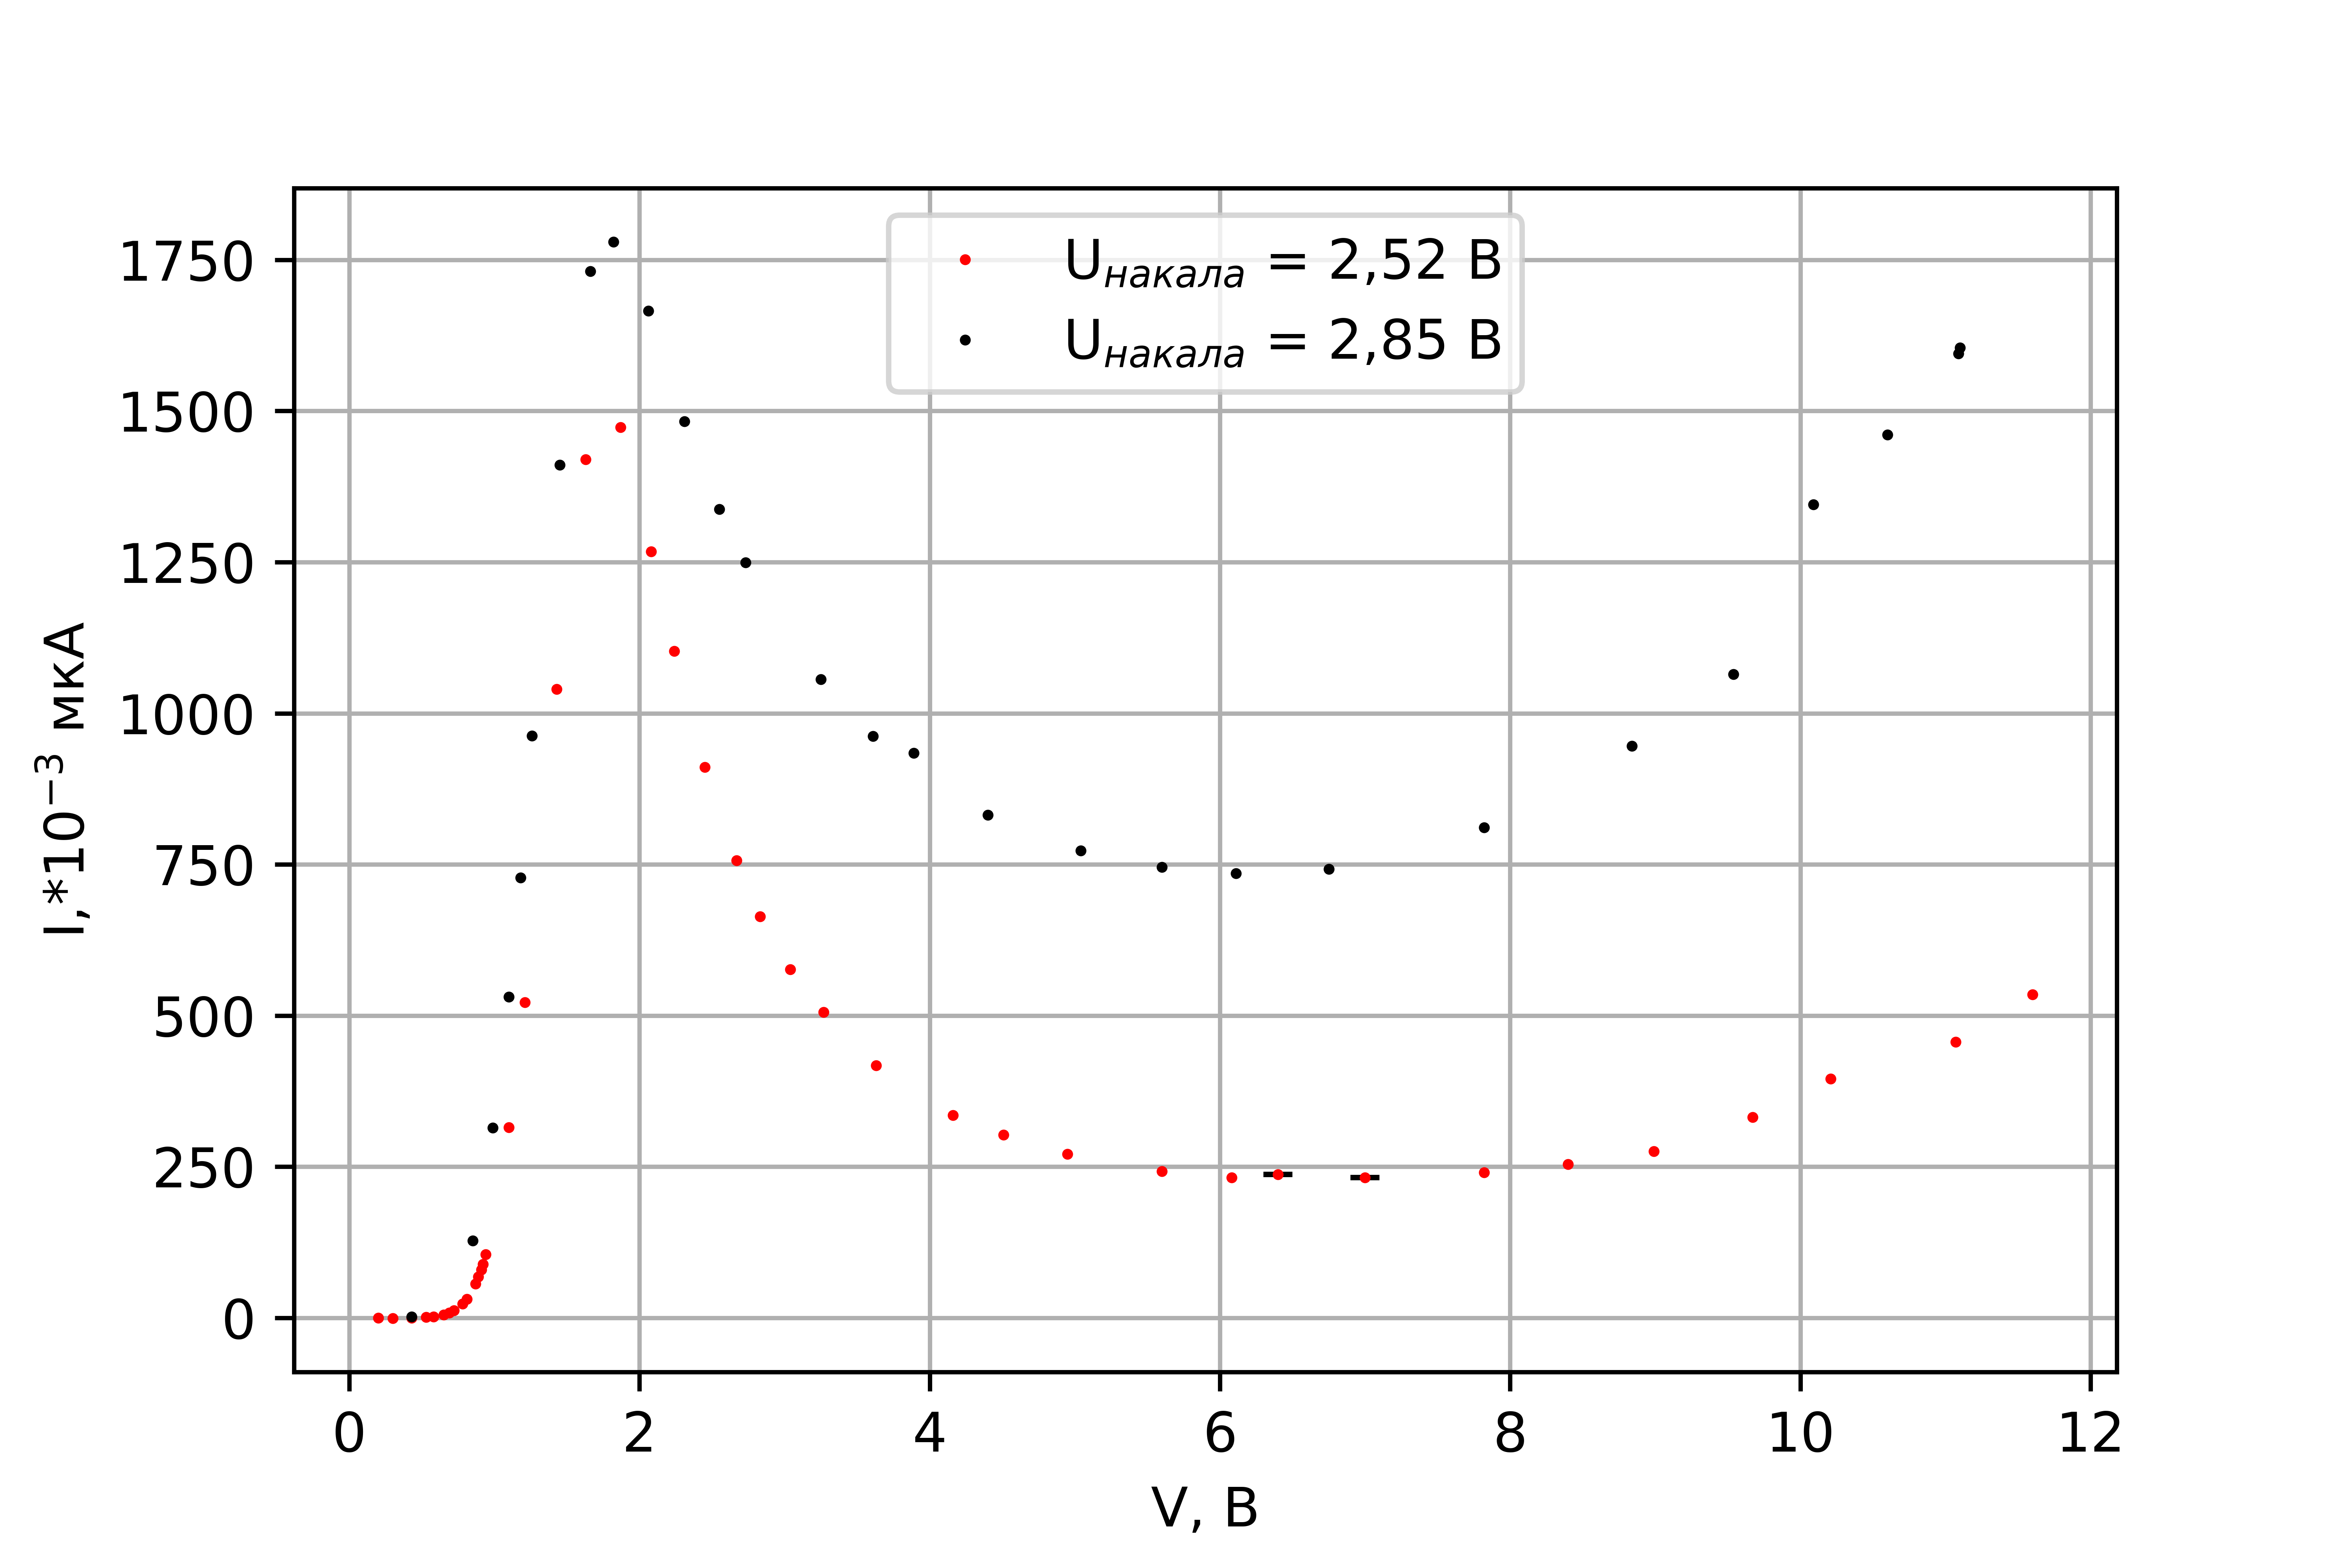
\includegraphics[width=14cm]{I(V).png}
    \caption{$I_{a} = f(V_{c})$}
    \label{fig:vac}
\end{figure}

Из ВАХ $I_{a} = f(V_{c})$, найдя $V_{max}$ и  $V_{min}$, получим:
\begin{equation*}
    l\approx (2,99\pm 0,32)\textup{~\AA}
\end{equation*}
\begin{equation*}
    U_0\approx (2,19\pm 0,13)\text{В}
\end{equation*}

Оценим, при каких напряжениях должны появляться максимумы в коэффициенте прохождения электронов для $n=2,3$ по формуле:
\begin{equation*}
    k_{2}l = \sqrt{\frac{2m(E_{n} + U_{0})}{\hslash^2}}l = \pi n
\end{equation*}

Откуда получаем $E_{n} = n^2(E_{1} + U_{0})-U_{0}$

Из последней формулы получим: $E_{2} = (27,1\pm3,8)$В, $E_{3} = (68,1\pm9,8)$В. Заметим, что полученные значения больше предела измерений прибора, поэтому увидеть 2 и 3 пики нам не удалось.

Найдем зависимость вероятности рассеяния электронов (с точностью до константы) от энергии с помощью формулы (5):

\begin{table}[H]
\begin{tabular}{|c|c|c|c|}
\hline
$Cw$   & $\sigma_{Cw}$ & $V$,В  & $\sigma_V$, В              \\ \hline
-    & -       & 0,20 & \multirow{21}{*}{0,01} \\ \cline{1-3}
-    & -       & 0,30 &                        \\ \cline{1-3}
-    & -       & 0,43 &                        \\ \cline{1-3}
7,40 & 0,11    & 0,53 &                        \\ \cline{1-3}
5,22 & 0,01    & 0,69 &                        \\ \cline{1-3}
6,60 & 0,05    & 0,58 &                        \\ \cline{1-3}
5,65 & 0,02    & 0,65 &                        \\ \cline{1-3}
4,80 & 0,01    & 0,72 &                        \\ \cline{1-3}
4,16 & 0,00    & 0,78 &                        \\ \cline{1-3}
3,86 & 0,00    & 0,81 &                        \\ \cline{1-3}
3,27 & 0,00    & 0,87 &                        \\ \cline{1-3}
3,08 & 0,00    & 0,89 &                        \\ \cline{1-3}
2,92 & 0,00    & 0,91 &                        \\ \cline{1-3}
2,81 & 0,00    & 0,92 &                        \\ \cline{1-3}
2,65 & 0,00    & 0,94 &                        \\ \cline{1-3}
1,54 & 0,00    & 1,10 &                        \\ \cline{1-3}
1,04 & 0,00    & 1,21 &                        \\ \cline{1-3}
0,35 & 0,00    & 1,43 &                        \\ \cline{1-3}
0,04 & 0,00    & 1,63 &                        \\ \cline{1-3}
0,00 & 0,00    & 1,87 &                        \\ \cline{1-3}
0,15 & 0,00    & 2,08 &                        \\ \hline
\end{tabular}
\hspace{1cm}
\begin{tabular}{|c|c|c|c|}
\hline
$Cw$   & $\sigma_{Cw}$ & $V$,В  & $\sigma_V$, В       \\ \hline
0,29 & 0,00    & 2,24  & \multirow{12}{*}{0,01} \\ \cline{1-3}
0,48 & 0,00    & 2,45  &                        \\ \cline{1-3}
0,67 & 0,00    & 2,67  &                        \\ \cline{1-3}
0,80 & 0,00    & 2,83  &                        \\ \cline{1-3}
0,94 & 0,00    & 3,04  &                        \\ \cline{1-3}
1,07 & 0,00    & 3,27  &                        \\ \cline{1-3}
1,26 & 0,00    & 3,63  &                        \\ \cline{1-3}
1,48 & 0,00    & 4,16  &                        \\ \cline{1-3}
1,58 & 0,00    & 4,51  &                        \\ \cline{1-3}
1,69 & 0,00    & 4,95  &                        \\ \cline{1-3}
1,80 & 0,00    & 5,60  &                        \\ \cline{1-3}
1,85 & 0,00    & 6,08  &                        \\ \hline
1,83 & 0,00    & 6,40  & \multirow{2}{*}{0,1}   \\ \cline{1-3}
1,85 & 0,00    & 7,00  &                        \\ \hline
1,81 & 0,00    & 7,82  & \multirow{7}{*}{0,01}  \\ \cline{1-3}
1,76 & 0,00    & 8,40  &                        \\ \cline{1-3}
1,68 & 0,00    & 8,99  &                        \\ \cline{1-3}
1,49 & 0,00    & 9,67  &                        \\ \cline{1-3}
1,32 & 0,00    & 10,21 &                        \\ \cline{1-3}
1,17 & 0,00    & 11,07 &                        \\ \cline{1-3}
1,01 & 0,00    & 11,60 &                        \\ \hline
\end{tabular}
\caption{Данные графика $Cw(V)$ для $U_{\text{накала}}=$ 2,52 В}
\end{table}

\begin{table}[H]
\begin{tabular}{|c|c|c|c|}
\hline
$Cw$   & $\sigma_{Cw}$ & $V$,В  & $\sigma_V$, В          \\ \hline
7,08 & 0,07    & 0,43 & \multirow{14}{*}{0,01} \\ \cline{1-3}
2,64 & 0,00    & 0,85 &                        \\ \cline{1-3}
1,73 & 0,00    & 0,99 &                        \\ \cline{1-3}
1,21 & 0,00    & 1,10 &                        \\ \cline{1-3}
0,89 & 0,00    & 1,18 &                        \\ \cline{1-3}
0,61 & 0,00    & 1,26 &                        \\ \cline{1-3}
0,23 & 0,00    & 1,45 &                        \\ \cline{1-3}
0,03 & 0,00    & 1,66 &                        \\ \cline{1-3}
0,00 & 0,00    & 1,82 &                        \\ \cline{1-3}
0,07 & 0,00    & 2,06 &                        \\ \cline{1-3}
0,18 & 0,00    & 2,31 &                        \\ \cline{1-3}
0,29 & 0,00    & 2,55 &                        \\ \cline{1-3}
0,35 & 0,00    & 2,73 &                        \\ \cline{1-3}
0,52 & 0,00    & 3,25 &                        \\ \hline
\end{tabular}
\hspace{1cm}
\begin{tabular}{|c|c|c|c|}
\hline
$Cw$   & $\sigma_{Cw}$ & $V$,В  & $\sigma_V$, В   \\ \hline
0,61 & 0,00    & 3,61  & \multirow{14}{*}{0,01} \\ \cline{1-3}
0,64 & 0,00    & 3,89  &                        \\ \cline{1-3}
0,76 & 0,00    & 4,40  &                        \\ \cline{1-3}
0,83 & 0,00    & 5,04  &                        \\ \cline{1-3}
0,87 & 0,00    & 5,60  &                        \\ \cline{1-3}
0,88 & 0,00    & 6,11  &                        \\ \cline{1-3}
0,87 & 0,00    & 6,75  &                        \\ \cline{1-3}
0,79 & 0,00    & 7,82  &                        \\ \cline{1-3}
0,63 & 0,00    & 8,84  &                        \\ \cline{1-3}
0,51 & 0,00    & 9,54  &                        \\ \cline{1-3}
0,28 & 0,00    & 10,09 &                        \\ \cline{1-3}
0,20 & 0,00    & 10,60 &                        \\ \cline{1-3}
0,10 & 0,00    & 11,10 &                        \\ \cline{1-3}
0,11 & 0,00    & 11,09 &                        \\ \hline
\end{tabular}
\caption{Данные графика $Cw(V)$ для $U_{\text{накала}}=$ 2,85 В}
\end{table}

Построим соответствующий график:

\begin{figure}[H]
    \centering
    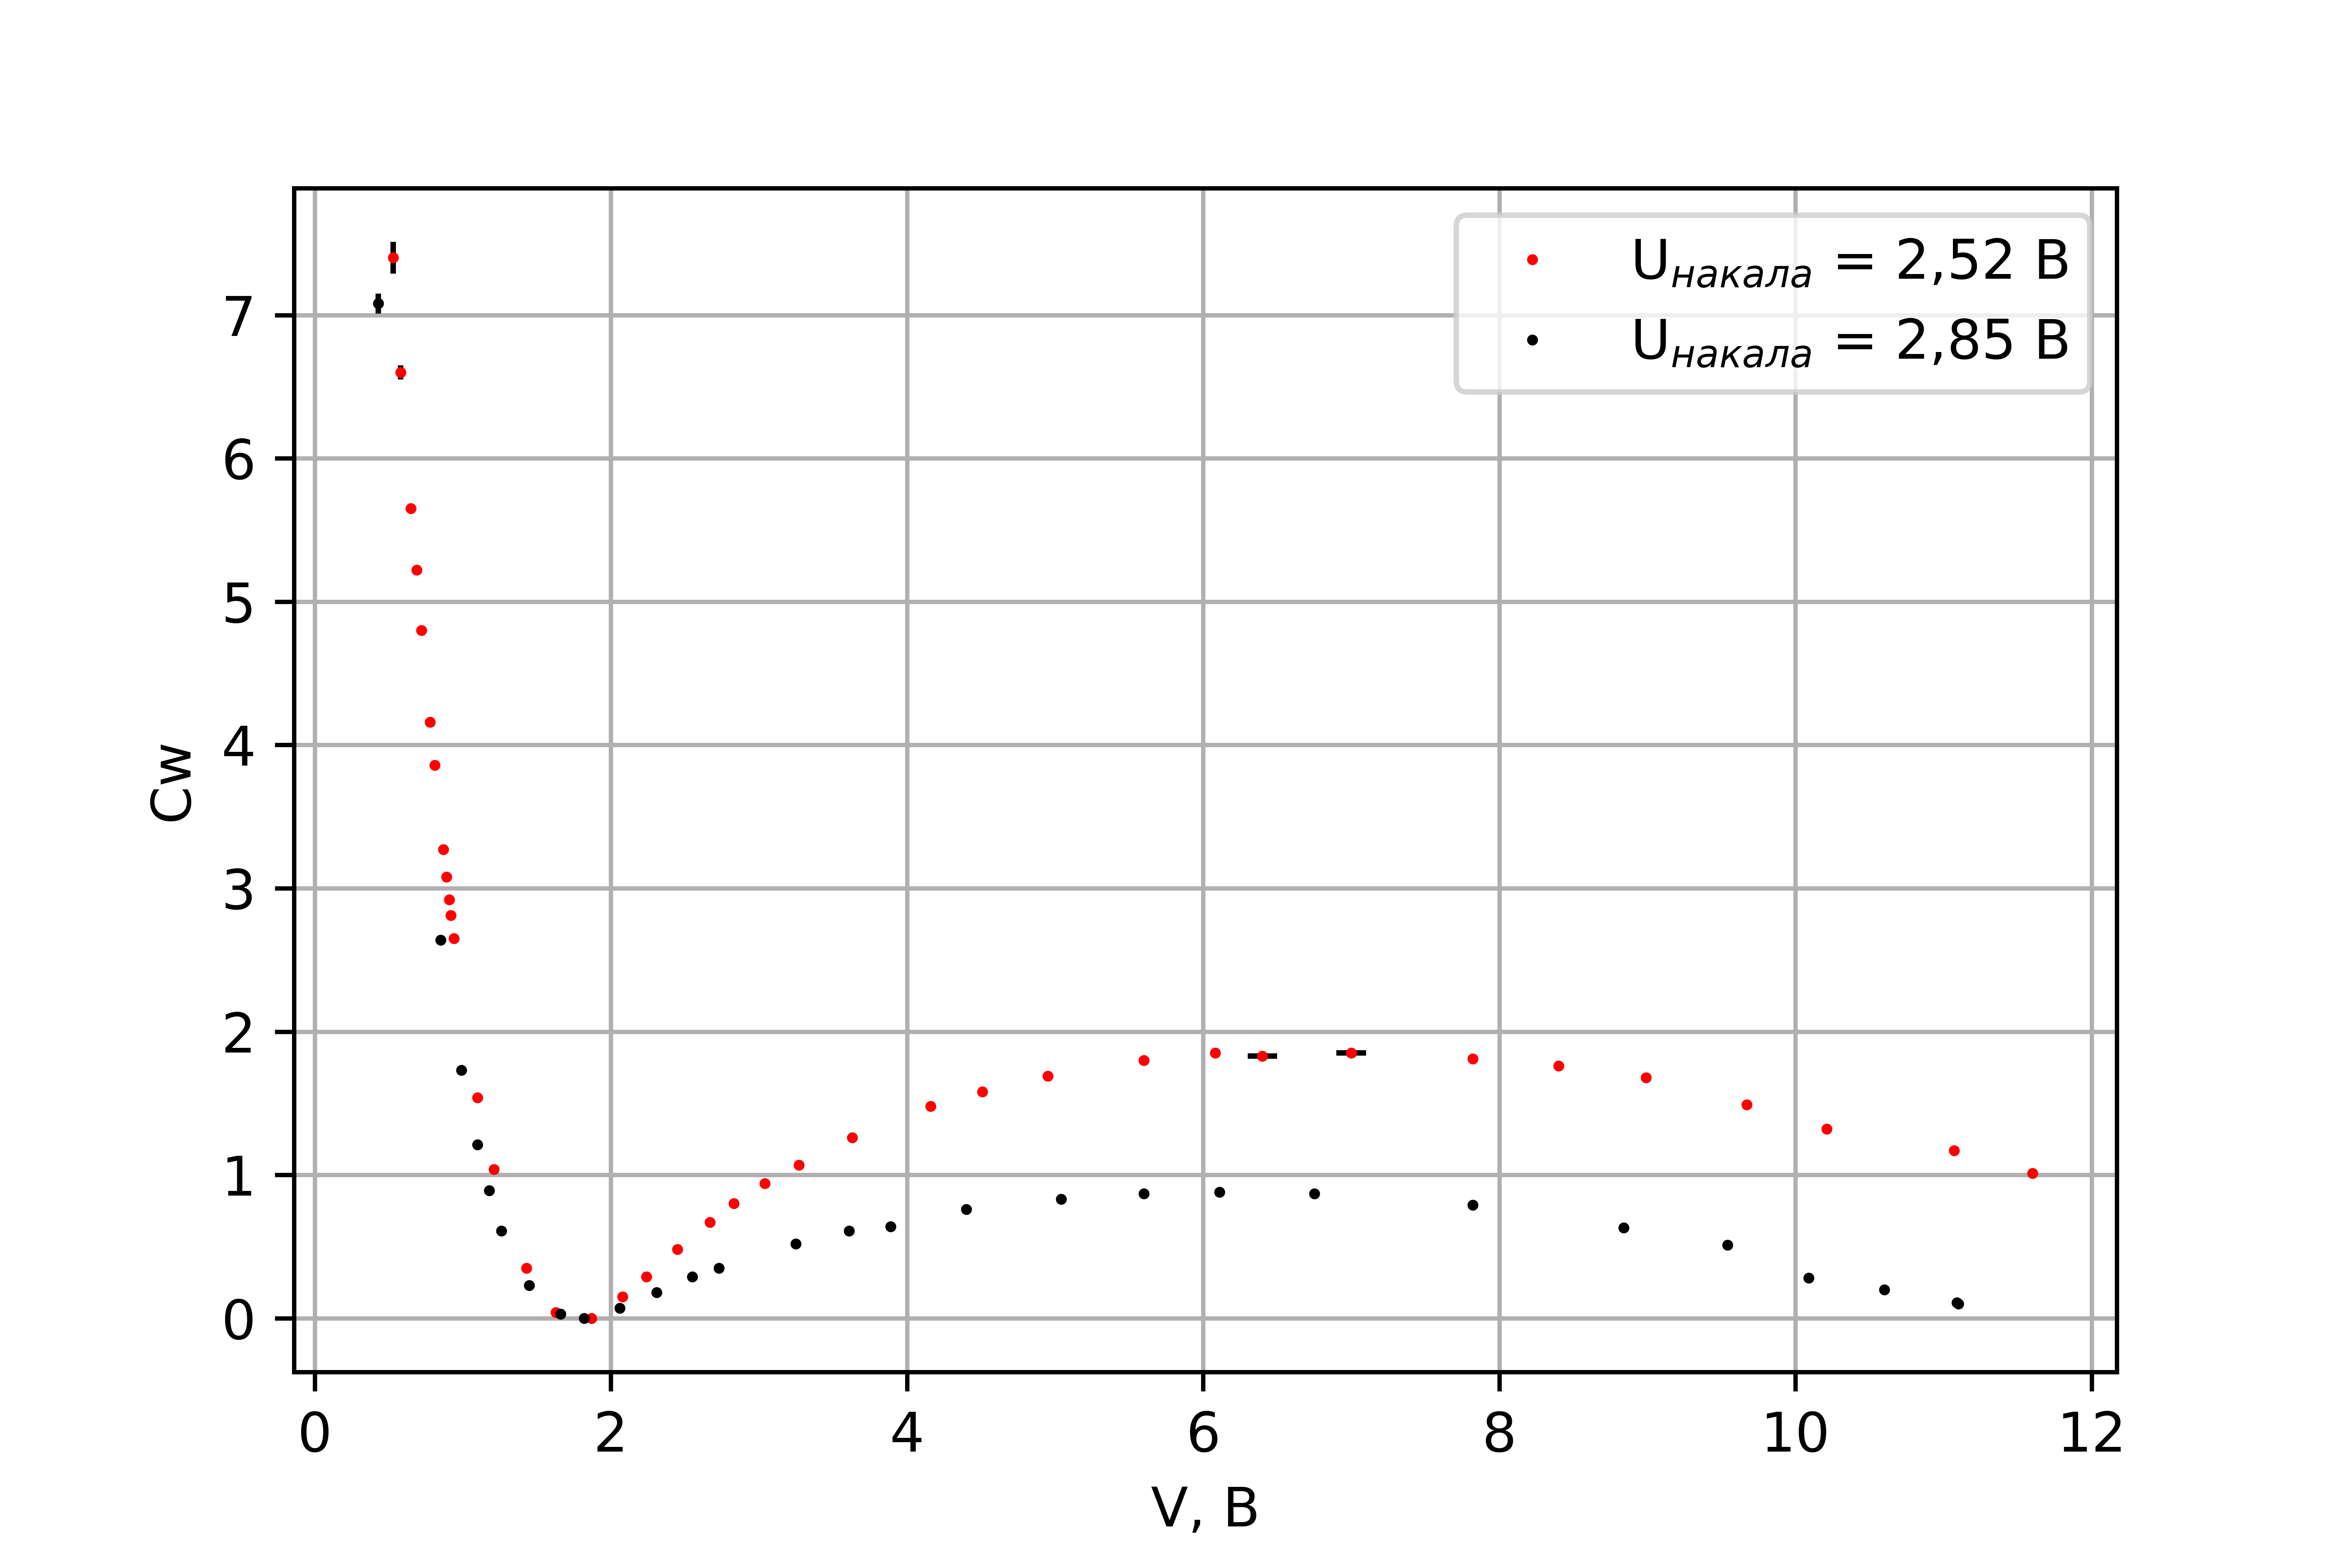
\includegraphics[width=14cm]{Cw(V).png}
    \caption{$Cw(V)$}
    \label{fig:vac}
\end{figure}

\section*{5. Выводы}
В ходе работы мы исследовали ВАХ тиратрона статическим и динамическим методами. Были получены ионизационный потенциал, радиус внешней оболочки атома инертного газа и глубина потенциальной ямы. По полученным значениям мы пришли к выводу, что тиратрон наполнен ксеноном.

\end{document}
